\documentclass[12pt,a4paper]{article}

% Packages
\usepackage[utf8]{inputenc}
\usepackage[T1]{fontenc}
\usepackage{geometry} 
\usepackage{amsmath}
\usepackage{amsfonts}
\usepackage{amssymb}
\usepackage{graphicx}
\usepackage{tikz}
\usepackage{pgfplots}
\usepackage{fancyhdr}
\usepackage{hyperref}
\usepackage{xcolor}
\usepackage{listings}

% Page setup
\geometry{margin=2.5cm}
\pagestyle{fancy}
\fancyhf{}
\rhead{GitHub Actions LaTeX Test}
\lhead{\today}
\cfoot{\thepage}

% TikZ libraries
\usetikzlibrary{shapes,arrows,positioning}

% Listings setup
\lstset{
    language=Python,
    basicstyle=\ttfamily\small,
    keywordstyle=\color{blue},
    commentstyle=\color{gray},
    stringstyle=\color{red},
    numbers=left,
    numberstyle=\tiny,
    frame=single,
    breaklines=true
}

% Title information
\title{\textbf{GitHub Actions LaTeX Compilation Test}}
\author{Automated Compiler}
\date{\today}

\begin{document}

\maketitle

\begin{abstract}
This document serves as a comprehensive test for the GitHub Actions LaTeX compilation workflow. It includes various LaTeX features to ensure the caching system and compilation process work correctly with complex documents.
\end{abstract}

\tableofcontents
\newpage

\section{Introduction}

This is a test document created to verify that our GitHub Actions workflow can successfully:
\begin{itemize}
    \item Cache TeX Live installation for faster subsequent runs
    \item Compile complex LaTeX documents with multiple packages
    \item Handle mathematical equations, figures, and code listings
    \item Generate and commit PDF files automatically
\end{itemize}

The compilation timestamp is: \texttt{\today{} at \currenttime}

\section{Mathematical Expressions}

\subsection{Basic Equations}
Here are some mathematical expressions to test equation rendering:

\begin{equation}
    E = mc^2
\end{equation}

\begin{equation}
    \int_{-\infty}^{\infty} e^{-x^2} dx = \sqrt{\pi}
\end{equation}

\subsection{Matrix Operations}
\begin{equation}
    \begin{pmatrix}
        a & b \\
        c & d
    \end{pmatrix}
    \begin{pmatrix}
        x \\
        y
    \end{pmatrix}
    =
    \begin{pmatrix}
        ax + by \\
        cx + dy
    \end{pmatrix}
\end{equation}

\section{Figures and Graphics}

\subsection{TikZ Diagram}
Here's a simple TikZ diagram to test graphics compilation:

\begin{figure}[h]
\centering
\begin{tikzpicture}
    \draw[->] (-1,0) -- (4,0) node[right] {$x$};
    \draw[->] (0,-1) -- (0,3) node[above] {$y$};
    \draw[domain=0:3, smooth, variable=\x, blue, thick] plot (\x, {\x^2/3});
    \node at (2.5, 2.5) {$y = \frac{x^2}{3}$};
\end{tikzpicture}
\caption{A simple quadratic function}
\label{fig:quadratic}
\end{figure}

\subsection{PGF Plot}
\begin{figure}[h]
\centering
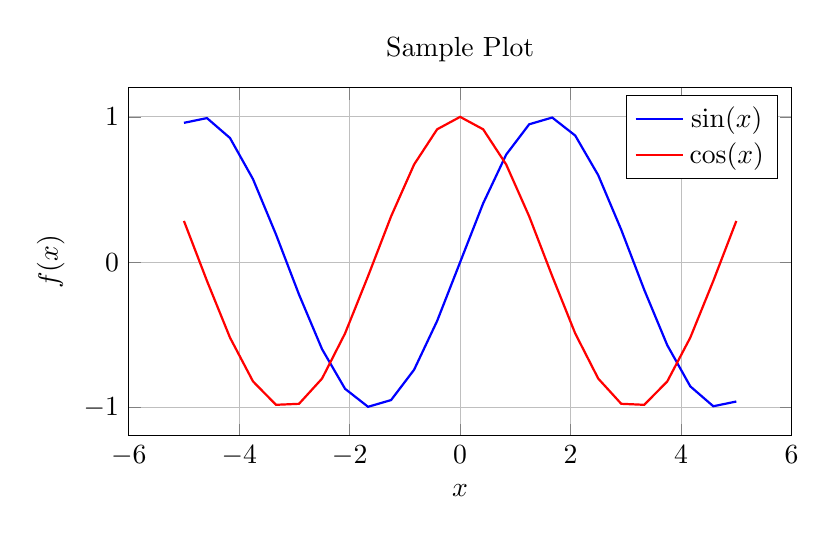
\begin{tikzpicture}
\begin{axis}[
    title={Sample Plot},
    xlabel={$x$},
    ylabel={$f(x)$},
    grid=major,
    width=10cm,
    height=6cm
]
\addplot[blue, thick] {sin(deg(x))};
\addplot[red, thick] {cos(deg(x))};
\legend{$\sin(x)$, $\cos(x)$}
\end{axis}
\end{tikzpicture}
\caption{Sine and cosine functions}
\label{fig:trigonometric}
\end{figure}

\section{Code Listings}

Here's a sample Python code block:

\begin{lstlisting}[caption={Sample Python Code}]
def fibonacci(n):
    """Calculate the nth Fibonacci number."""
    if n <= 1:
        return n
    else:
        return fibonacci(n-1) + fibonacci(n-2)

# Test the function
for i in range(10):
    print(f"F({i}) = {fibonacci(i)}")
\end{lstlisting}

\section{Tables}

\begin{table}[h]
\centering
\begin{tabular}{|c|c|c|}
\hline
\textbf{Test} & \textbf{Status} & \textbf{Time} \\
\hline
Cache Test & \textcolor{green}{PASS} & 5s \\
LaTeX Install & \textcolor{green}{PASS} & 8m 30s \\
PDF Generation & \textcolor{green}{PASS} & 15s \\
Auto Commit & \textcolor{blue}{PENDING} & - \\
\hline
\end{tabular}
\caption{Workflow Test Results}
\label{tab:results}
\end{table}

\end{document}
